\documentclass[aspectratio=169, 10pt]{beamer}

% --- Packages ---
\usepackage[utf8]{inputenc}
\usepackage[T1]{fontenc}
\usepackage[english]{babel}
\usepackage{graphicx}
\usepackage{amsmath, amssymb}
\usepackage{listings}
\usepackage{xcolor}
\usepackage{tikz}

% --- Configuration du code ---
\definecolor{codegreen}{rgb}{0,0.6,0}
\definecolor{backcolour}{rgb}{0.95,0.95,0.92}
\lstdefinestyle{python}{
    backgroundcolor=\color{backcolour},   
    commentstyle=\color{codegreen},
    keywordstyle=\color{blue},
    basicstyle=\ttfamily\tiny,
    breaklines=true,                 
    captionpos=b,                    
    keepspaces=true,                 
    language=Python
}
\lstset{style=python}

% --- Thème ---
\usetheme{Madrid}
\usecolortheme{seahorse}
\setbeamertemplate{navigation symbols}{}

% --- MÉTADONNÉES ---
\title[Grover $\&$ Quantum Counting]{Grover’s Search and Quantum Counting}
\subtitle{Project 6 - PHYS-541 Quantum Computing}
\author[Victor Peucelle]{Presented by: Victor Peucelle} % Prénom Nom est standard en anglais
\institute[EPFL]{
    \textbf{École Polytechnique Fédérale de Lausanne}\\
    Academic Year: 2025--2026
    \vspace{0.2cm}
    
    \tiny
    Professor: Vincenzo Savona \\
    Assistants: Sara Alves dos Santos, David Linteau, Shao Chiew
}
\date{\today}

\begin{document}

% ---------------------------------------------------------
% SLIDE DE TITRE
% ---------------------------------------------------------
\begin{frame}
    \titlepage
\end{frame}

% ---------------------------------------------------------
% INTRODUCTION / PLAN
% ---------------------------------------------------------
\begin{frame}{Project Overview $\&$ Objectives}
    This project focuses on the implementation and analysis of Grover's Search and Quantum Counting algorithms.
    
    \vspace{0.5cm} % 1cm était trop grand

    \begin{enumerate}
        \item \textbf{Theory:} Detailed explanation of Grover's algorithm and Quantum Counting (based on Nielsen $\&$ Chuang).
        \item \textbf{Complexity:} Analysis of quantum speedup limits and NP complexity class.
        \item \textbf{Implementation:} Construction of Oracles (with and without Ancilla) on IBM Qiskit.
        \item \textbf{Noise Analysis:} Performance study under simulated noise and circuit depth limitations.
    \end{enumerate}
\end{frame}

% =========================================================
% PARTIE 1: THÉORIE (Requirement 1)
% =========================================================
\section{Theory: Grover $\&$ Counting}

\begin{frame}{1. Grover's Algorithm: The Mechanism}
    \textbf{Goal:} Find marked element(s) $x$ such that $f(x)=1$ in a database of size $N=2^n$.
    
    \vspace{0.5cm}

    \begin{columns}
        \column{0.55\textwidth}
        The algorithm iterates the \textbf{Grover Operator} $G = (2|\psi\rangle\langle\psi| - I)O$:
        \begin{itemize}
            \item \textbf{Oracle ($O$):} Flips the phase of the solution $|x\rangle$.
            \item \textbf{Diffuser:} Inversion about the mean.
        \end{itemize}
        
        \vspace{0.2cm}
        \textbf{Geometric Interpretation:}
        Rotates the state vector by angle $\theta$ towards the target state $|\beta\rangle$.
        $$ \theta \approx 2\sqrt{m/N} $$
        
        \column{0.45\textwidth}
        \begin{center}
            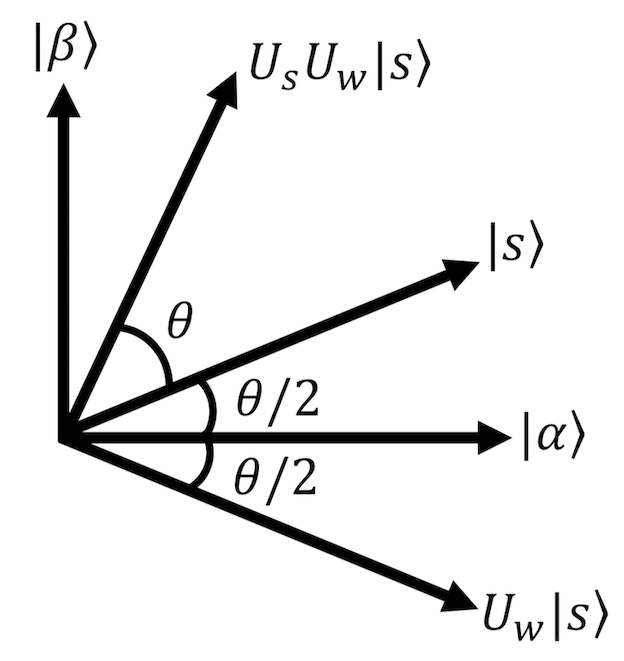
\includegraphics[width=0.6\textwidth]{../asset/grover_geometry.png}
        \end{center}
    \end{columns}
\end{frame}

\begin{frame}{Circuit Implementation ($n=3$)}
    \begin{center}
        % L'image du circuit
        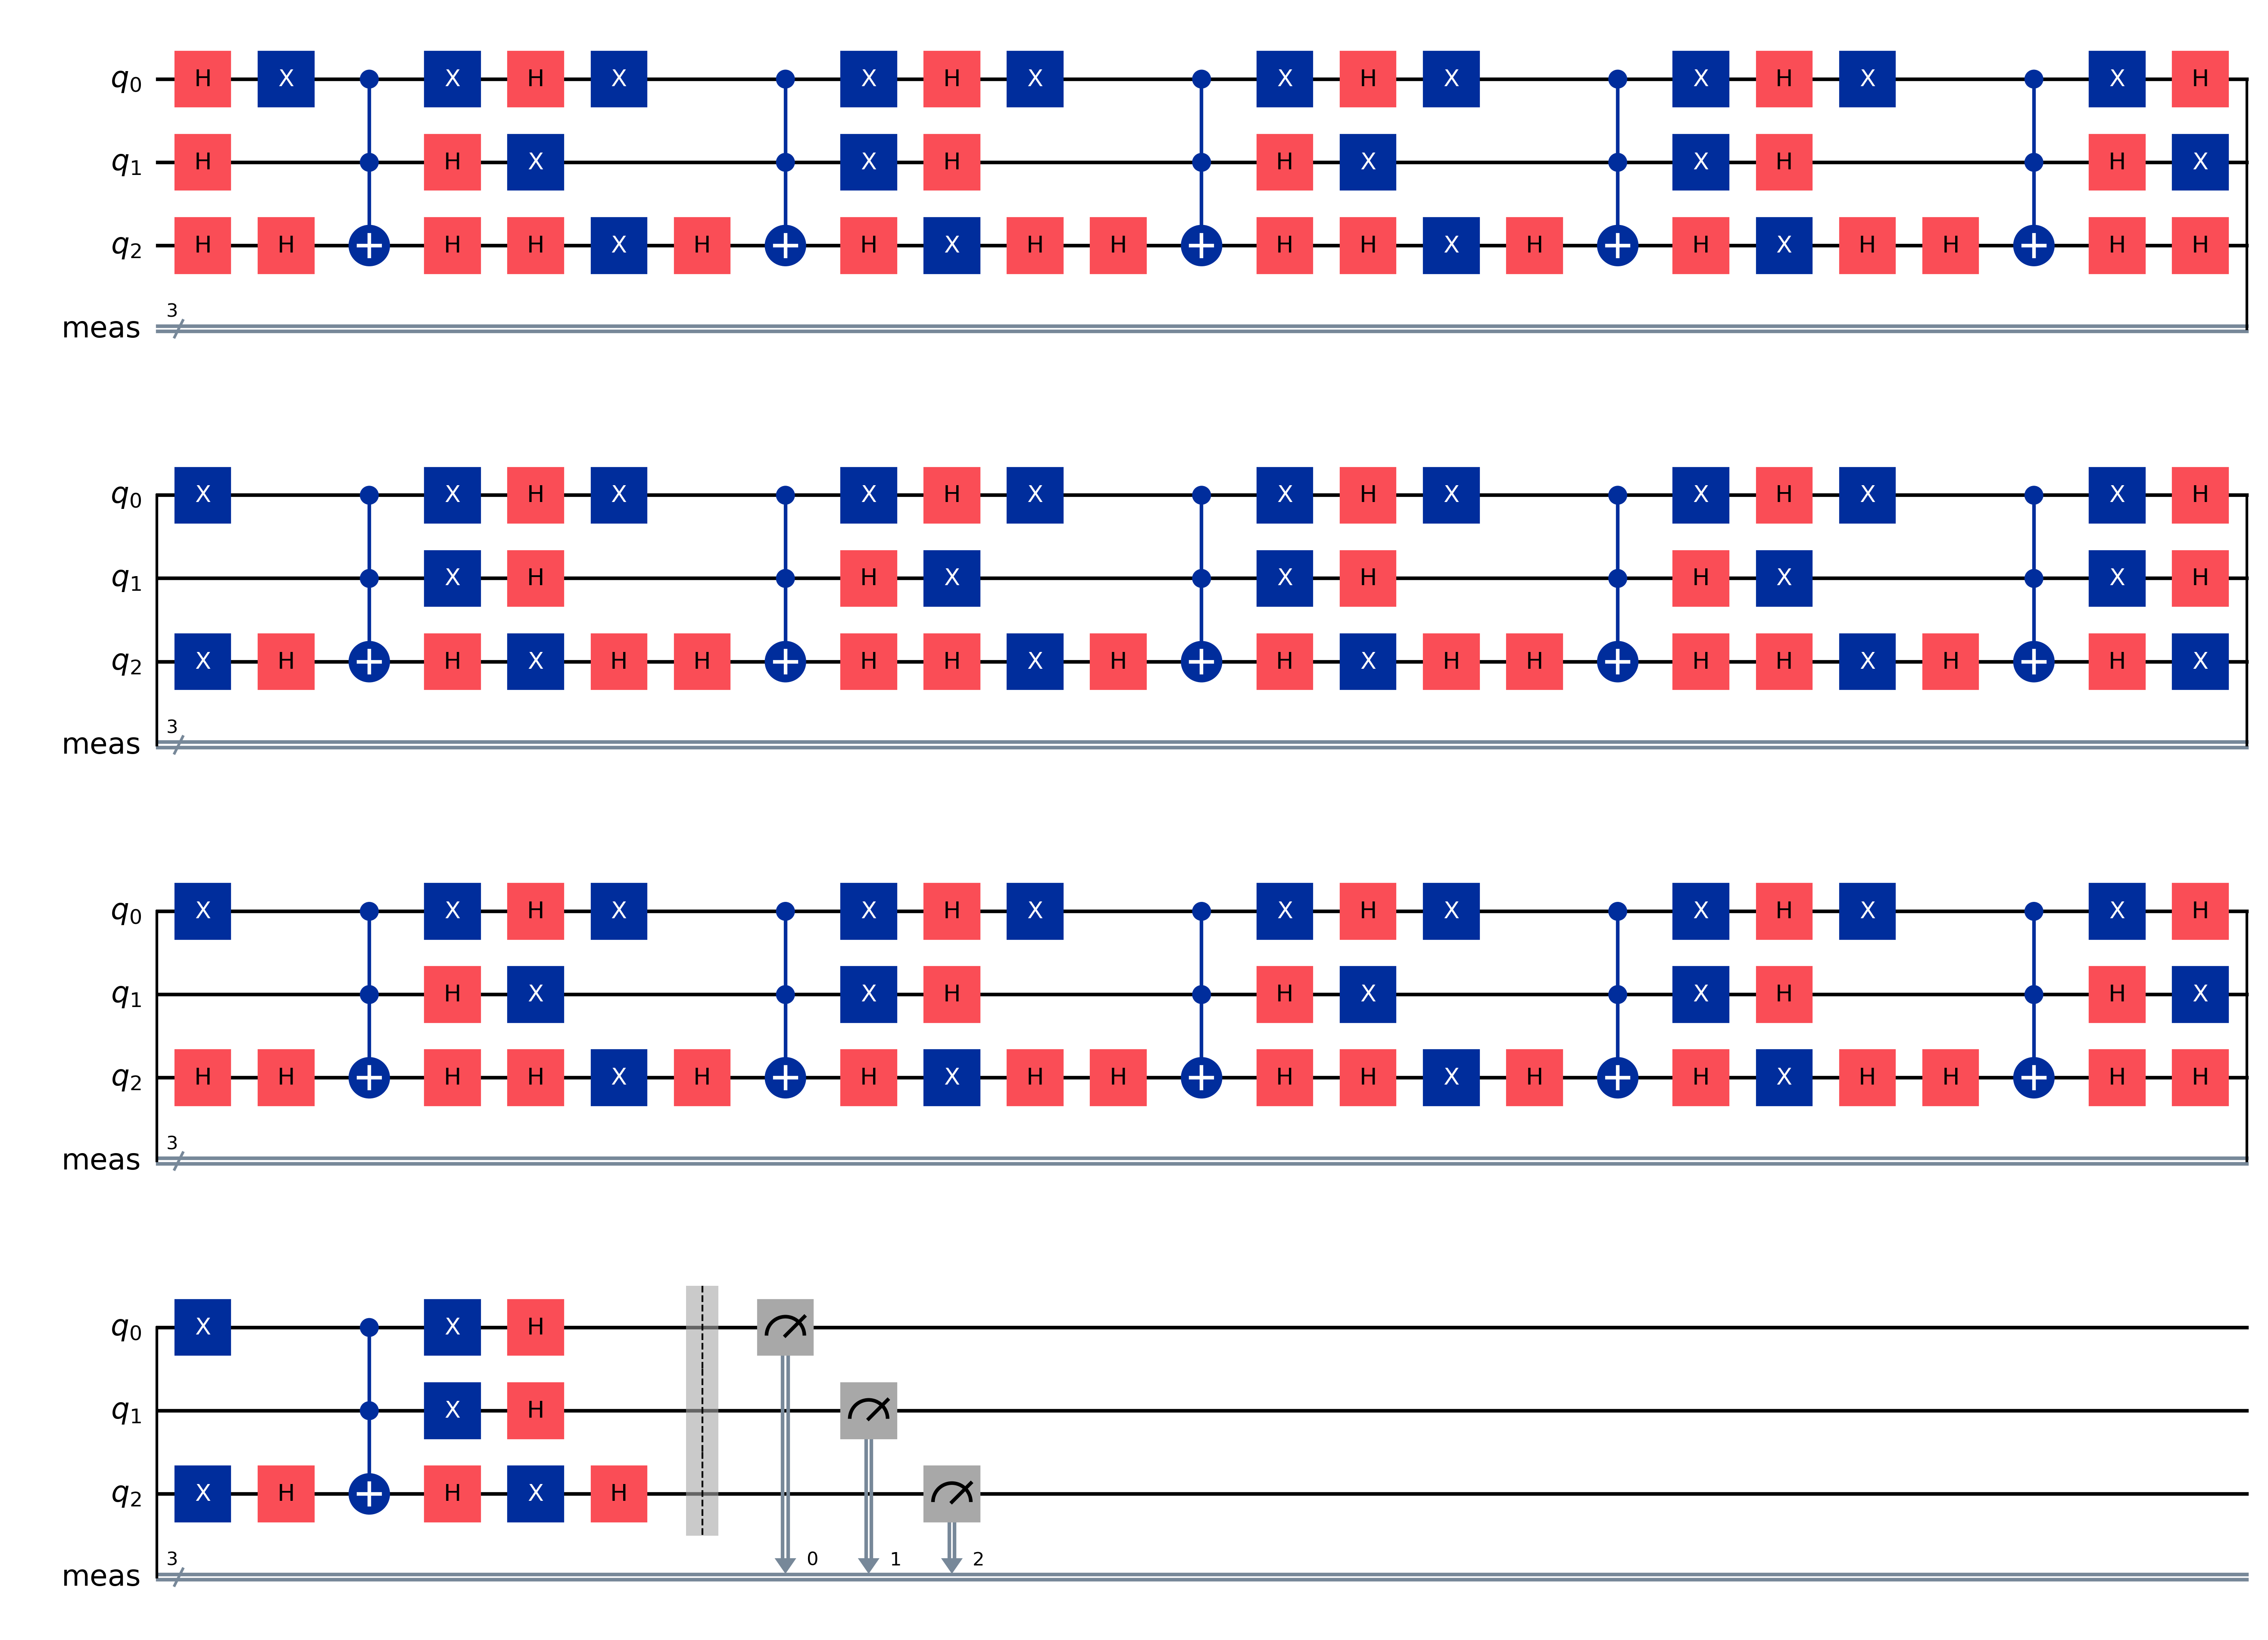
\includegraphics[width=\textwidth, height=0.55\textheight, keepaspectratio]{../asset/circuit_grover_draw.png}
    \end{center}

    \vspace{0.2cm}

    % Légende explicative alignée avec les étapes du circuit
    \begin{columns}[t]
        \column{0.33\textwidth}
        \centering
        \textbf{1. Initialization} \\
        \footnotesize Apply $H^{\otimes n}$ to create equal superposition of all $N=8$ states.
        
        \column{0.33\textwidth}
        \centering
        \textbf{2. Oracle ($U_w$)} \\
        \footnotesize Flips the phase of the target state (e.g., $|101\rangle$).
        
        \column{0.33\textwidth}
        \centering
        \textbf{3. Diffuser ($U_s$)} \\
        \footnotesize Inversion about the mean. Increases amplitude of the marked state.
    \end{columns}
\end{frame}

\begin{frame}{Theoretical Performance}
    \textbf{Number of Iterations:} 
    To maximize the probability of measuring a marked state, perform:
    $$ r \approx \frac{\pi}{4}\sqrt{\frac{N}{m}} $$
    
    \vspace{0.2cm}
    \textbf{Probability of Success After $r$ Iterations:}
    $ P_{\text{success}} = \sin^2\left((2r + 1)\frac{\theta}{2}\right) $
    
    \begin{columns}
        \column{0.5\textwidth}
        \textbf{Example:} $n=3$ ($N=8$), $m=1$:
        \begin{itemize}
            \item $\theta \approx 0.707$ radians.
            \item Optimal iterations: $r \approx 1$.
            \item $P_{\text{success}} \approx 1$.
        \end{itemize}

        \column{0.5\textwidth}
        \begin{center}
            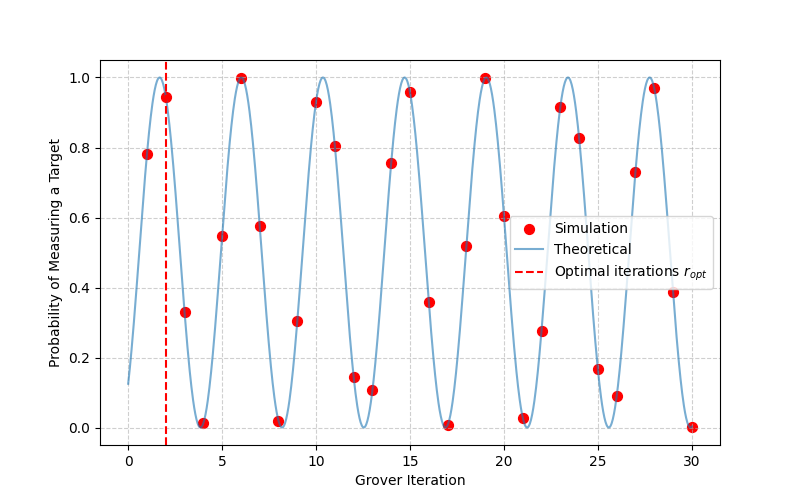
\includegraphics[width=\textwidth]{../asset/grover_simulated_probability_n3_m1.png}
        \end{center}
    \end{columns}
\end{frame}

% --- DÉPLACÉ ICI : La théorie du Counting AVANT les résultats ---
\begin{frame}{1. Quantum Counting Algorithm}
    \textbf{Problem:} Grover's optimal iterations $r$ depend on $m$. What if $m$ is unknown?
    
    \begin{block}{The Solution}
        Combine Grover operator $G$ with \textbf{Quantum Phase Estimation (QPE)}.
    \end{block}
    
    \begin{itemize}
        \item The eigenvalues of $G$ are $e^{\pm i\theta}$.
        \item QPE estimates the phase $\theta$.
        \item Since $\sin(\theta/2) = \sqrt{m/N}$, we can deduce $m$:
        $$ m \approx N \sin^2(\theta/2) $$
    \end{itemize}
\end{frame}

\begin{frame}{Quantum Counting on Real Hardware (IBM Turing)}
    % --- 1. Contexte Expérimental (Bandeau du haut) ---
    \begin{block}{Experimental Setup}
        \footnotesize
        \begin{itemize}
            \item \textbf{Backend:} \texttt{ibm\_turing} (127-qubit Eagle processor).
            \item \textbf{Parameters:} $n=3$ (Search Space), 2000 Shots.
            \item \textbf{Objective:} Estimate $m$ (number of solutions) via Phase Estimation.
        \end{itemize}
    \end{block}

    \vspace{0.2cm}

    % --- 2. Les Graphiques ---
    \begin{columns}
        \column{0.5\textwidth}
        \centering
        \textbf{Experiment A: 1 Solution} \\
        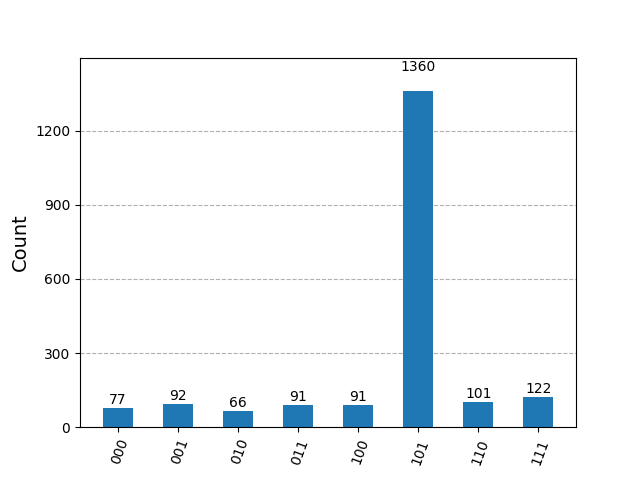
\includegraphics[width=\textwidth, height=4cm, keepaspectratio]{../asset/IBM/counting_1.png}
        \\ \tiny{Measured Phase Distribution ($m=1$)}
        
        \column{0.5\textwidth}
        \centering
        \textbf{Experiment B: 2 Solutions} \\ % Ou changez le titre selon vos images
        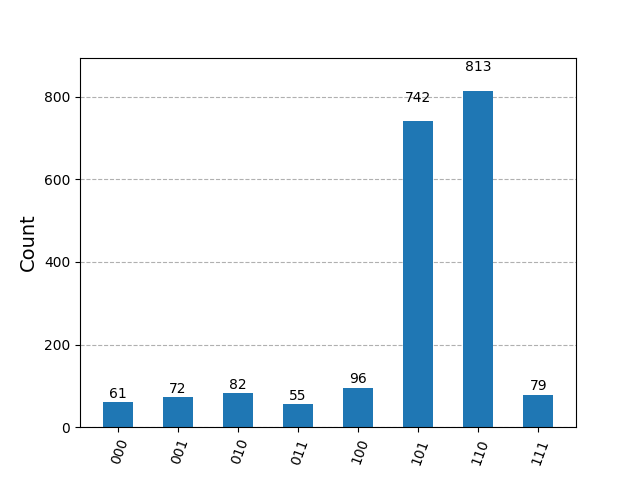
\includegraphics[width=\textwidth, height=4cm, keepaspectratio]{../asset/IBM/counting_2.png}
        \\ \tiny{Measured Phase Distribution ($m=2$)}
    \end{columns}

    \vspace{0.3cm}

    % --- 3. Observation / Conclusion ---
    \begin{alertblock}{Analysis}
        \footnotesize
        Despite hardware noise (readout errors $\&$ decoherence), distinct peaks are visible.
        The algorithm successfully identifies different phase values $\theta$ for different solution counts.
    \end{alertblock}
\end{frame}

% =========================================================
% PARTIE 2: COMPLEXITÉ & NP (Requirement 2)
% =========================================================
\section{Complexity Analysis}

\begin{frame}{2. Grover and Computational Complexity}
    \textbf{Quadratic Speedup vs Exponential Speedup}
    \begin{itemize}
        \item Classical Search: $\mathcal{O}(N)$
        \item Grover Search: $\mathcal{O}(\sqrt{N})$
    \end{itemize}
    
    \vspace{0.5cm}
    \textbf{Can Grover solve NP-Complete problems efficiently?}
    \begin{alertblock}{Limitation}
        NP-Complete problems (like SAT) have search spaces of size $N=2^n$.
        \begin{itemize}
            \item Brute force: $2^n$ operations.
            \item Grover: $\sqrt{2^n} = 2^{n/2}$ operations.
        \end{itemize}
        While $2^{n/2}$ is a significant improvement, it is \textbf{still exponential}. Grover does not place NP-complete problems into the BQP class.
    \end{alertblock}
\end{frame}

\begin{frame}{Failure of QPE on Real Hardware}
    \begin{columns}
        \column{0.4\textwidth}
        \begin{center}
            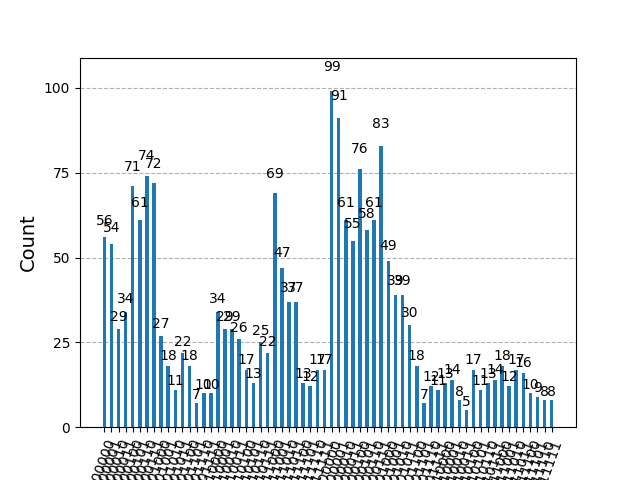
\includegraphics[width=\textwidth]{../asset/IBM/counting_qpe_1.png}
        \end{center}
        
        \column{0.6\textwidth}
        \small
        \textbf{Observation:}
        While Grover's Search ($\mathcal{O}(\sqrt{N})$ depth) yielded results on IBM Heron, Quantum Counting produced uniform noise.
        
        \vspace{0.2cm}
        \textbf{Why?}
        \begin{itemize}
            \item QPE requires applying Controlled-$G^{2^k}$.
            \item Controlling the Grover operator drastically increases the CNOT count.
            \item Total depth exceeds the qubit coherence time ($T_2$).
        \end{itemize}
        
        \begin{block}{Conclusion}
             Gap between 'Search' (NISQ-friendly) and 'Estimation' (Requires Error Correction).
        \end{block}
    \end{columns}
\end{frame}

\begin{frame}{Quantum Counting Results (Simulation)}
    \textbf{Setup:} 
    \begin{itemize}
        \item Search space: $n=3$ qubits ($N=8$).
        \item Precision: $t=6$ counting qubits (allows distinguishing phases with accuracy $2^{-6}$).
        \item Noise Model: Depolarizing error ($\epsilon = 10^{-5}$).
    \end{itemize}

    \begin{center}
        % L'image occupe 75% de la hauteur dispo pour être bien visible
        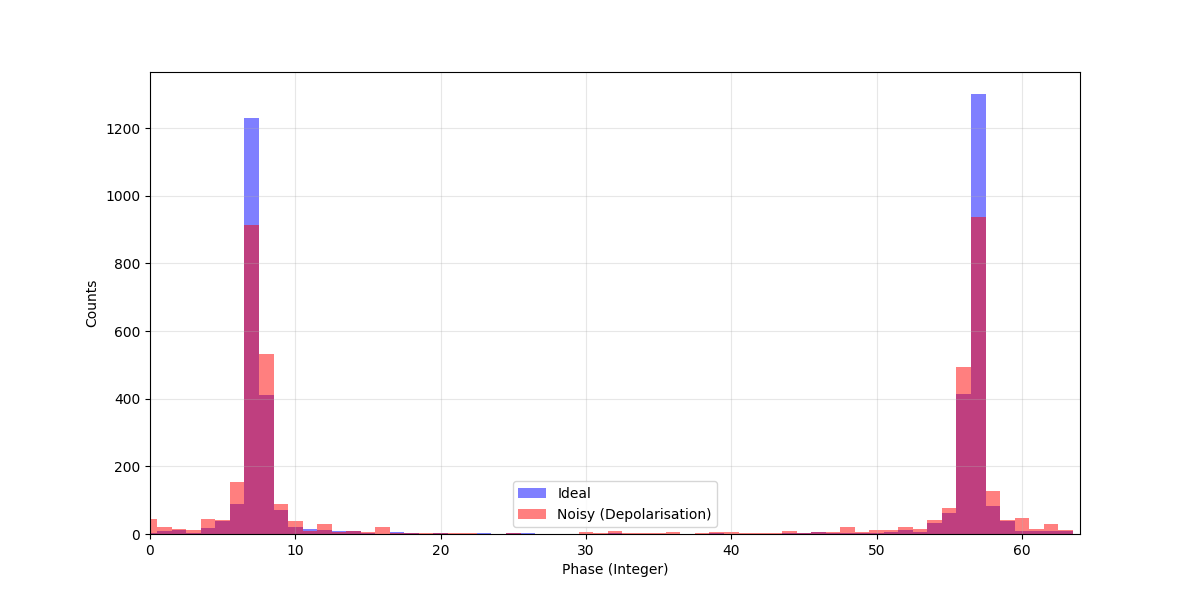
\includegraphics[height=0.55\textheight, keepaspectratio]{../asset/quantum_counting_ideal_vs_noisy_n3_t6.png}
    \end{center}

    \footnotesize
    \textbf{Observation:} 
    The dominant peak corresponds to the eigenvalue $\theta$. Using the formula $m \approx N \sin^2(\theta/2)$, the algorithm correctly identifies the number of solutions $m$, even with simulated noise.
\end{frame}

% =========================================================
% PARTIE 3: IMPLÉMENTATION (Requirement 3)
% =========================================================
\section{Implementation (Qiskit)}

\begin{frame}[fragile]{3. Oracle Implementation Strategy}
    \textbf{Task:} Implement $f(x)=1$ for $m=1$ or $m=2$ targets.
    
    We explored two approaches for the Multi-Controlled-X (MCX) gates:
    \vspace{0.5cm}
    
    \begin{columns}
        \column{0.5\textwidth}
        \textbf{A. With Ancilla Qubits}
        \begin{itemize}
            \item Uses extra qubits to decompose Toffoli gates.
            \item \textbf{Pros:} Linear depth scaling $\mathcal{O}(n)$.
            \item \textbf{Cons:} Requires more qubits.
        \end{itemize}
        
        \column{0.5\textwidth}
        \textbf{B. Without Ancilla}
        \begin{itemize}
            \item Uses complex decompositions of MCX gates.
            \item \textbf{Pros:} Saves qubits.
            \item \textbf{Cons:} Depth grows exponentially, creating massive noise.
        \end{itemize}
    \end{columns}
\end{frame}

\begin{frame}{3. Hardware Complexity: The Cost of Connectivity}
    \begin{columns}
        % --- Colonne de Gauche : Graphique ---
        \column{0.40\textwidth}
        \centering
        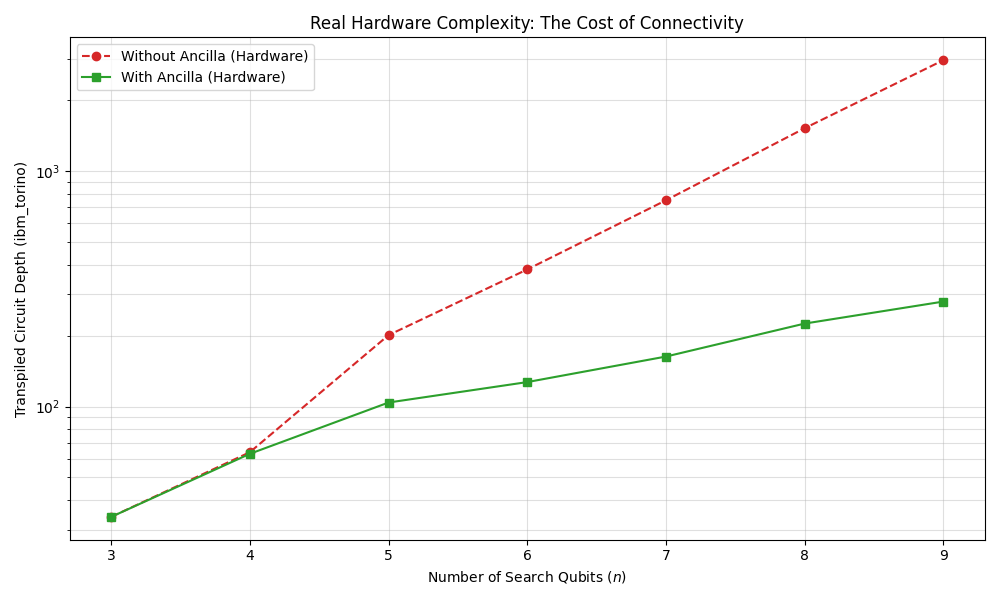
\includegraphics[width=\textwidth, height=0.75\textheight, keepaspectratio]{../asset/IBM/oracle_complexity_real_fixed.png}

        \vspace{0.2cm}

        \textbf{Experimental Setup:}
        \begin{itemize}
            \item \textbf{Backend:} \texttt{ibm\_torino} (133-qubit Heron).
            \item \textbf{Metric:} Transpiled Depth (Log Scale).
            \item \textbf{Optimization Level:} 3 (Max).
        \end{itemize}
        
        % --- Colonne de Droite : Analyse ---
        \column{0.55\textwidth}
        
        \textbf{Analysis:}
        \begin{enumerate}
            \item \textcolor{red}{\textbf{No Ancilla (Red):}} 
            Uses \texttt{MCXGrayCode}. Depth grows exponentially.
            \item \textcolor{green!60!black}{\textbf{With Ancilla (Green):}} 
            Uses \texttt{MCXVChain}. Depth grows linearly.
        \end{enumerate}
        
        \vspace{0.2cm}
        
        \begin{alertblock}{Key Finding}
            Without ancillas, the transpiler must insert massive amounts of \textbf{SWAP gates} to satisfy the limited connectivity of the chip, making the circuit useless for $n > 5$.
        \end{alertblock}
    \end{columns}
\end{frame}

% =========================================================
% PARTIE 4: BRUIT & PERF (Requirement 4)
% =========================================================
\section{Noise Analysis}

\begin{frame}{4. Hardware Performance: Grover Oscillations}
    \begin{columns}
        % --- Colonne de Gauche : Le Plot ---
        \column{0.50\textwidth}
        \centering
        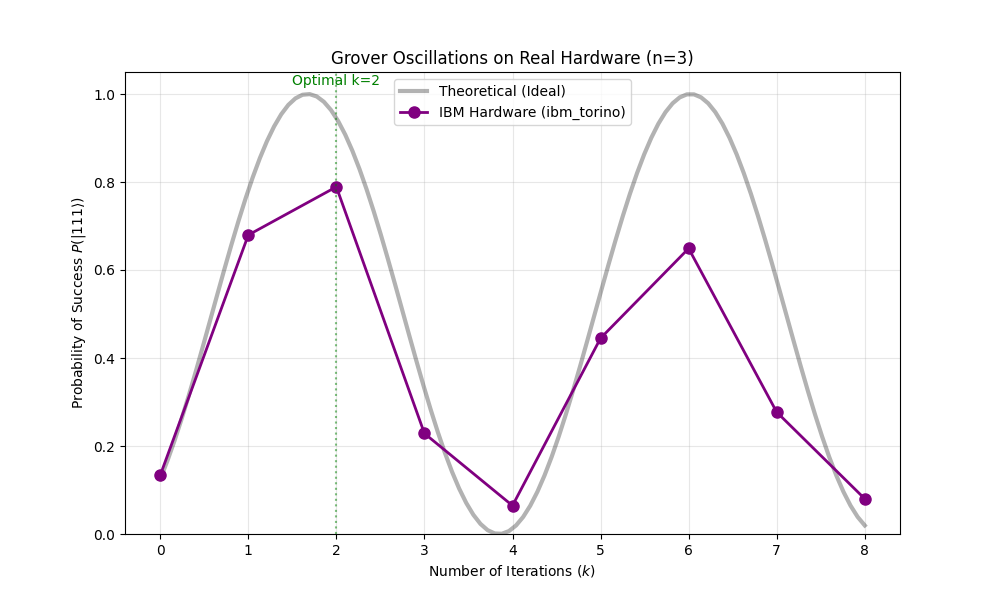
\includegraphics[width=\textwidth, height=0.75\textheight, keepaspectratio]{../asset/IBM/grover_oscillations_hardware_vs_theory.png}
        \textbf{Experimental Protocol:}
        \begin{itemize}
            \item \textbf{Target:} $|111\rangle$ ($n=3$).
            \item \textbf{Shots:} 2000 per iteration step.
            \item \textbf{Transpilation:} Optimization Level 3 (Aggressive gate reduction).
        \end{itemize}
        
        % --- Colonne de Droite : Analyse ---
        \column{0.50\textwidth}
        
        \textbf{Key Observations:}
        \begin{enumerate}
            \item \textbf{Validation:} The hardware (purple) closely follows the theoretical sinusoidal curve (black).
            \item \textbf{Optimal Peak:} Maximum probability occurs at $k=2$, matching the theory exactly.
            \item \textbf{Damping:} The peak $< 1.0$ and decays over time. As $k$ increases, circuit depth increases, accumulating gate errors and decoherence.
        \end{enumerate}
    \end{columns}
\end{frame}

\begin{frame}{4. Performance Under Noise}
    \textbf{The Challenge:} 
    Small $\theta/2 \approx \sqrt{m/N}$ implies large number of iterations $r$.
    $$ \text{Circuit Depth} \propto r \times \text{Oracle Depth} $$
    
    \begin{columns}
        \column{0.5\textwidth}
        \textbf{Simulation Results:}
        \begin{itemize}
            \item For small $n$ ($n \le 4$): High fidelity.
            \item For larger $n$: Success probability drops below classical threshold.
            \item \textbf{Limit:} On current NISQ models, coherence time limits usage to small instances.
        \end{itemize}
        
        \column{0.5\textwidth}
        \begin{center}
            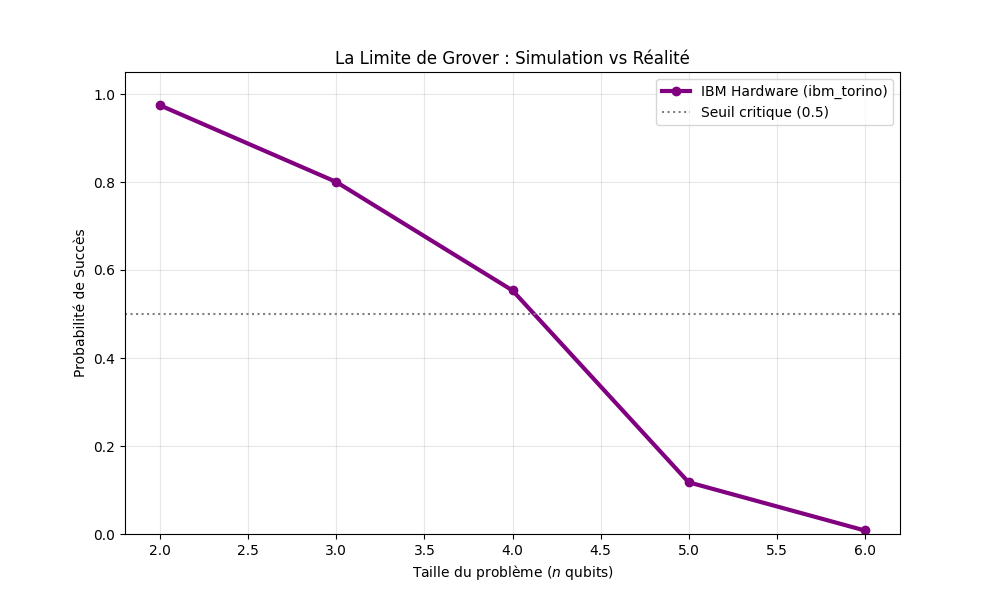
\includegraphics[width=\textwidth]{../asset/IBM/grover_hardware_vs_simulation.png}
        \end{center}
    \end{columns}
\end{frame}

\begin{frame}{4. Noise Impact: Stability Range Analysis}
    \begin{columns}
        % Colonne de gauche : Explications
        \column{0.45\textwidth}
        
        \vspace{0.5cm}
        \textbf{The "Tipping Point" (Red Boxes):}
        \begin{itemize}
            \item Highlighted cells indicate $P \approx 0.5$.
            \item This is the \textbf{critical threshold}. Beyond this line (top-right), noise dominates the quantum signal.
            \item \textbf{Observation:} For current hardware error rates ($\sim 10^{-2}$), we are limited to very small $n$.
        \end{itemize}

        % Colonne de droite : L'image
        \column{0.55\textwidth}
        \begin{center}
            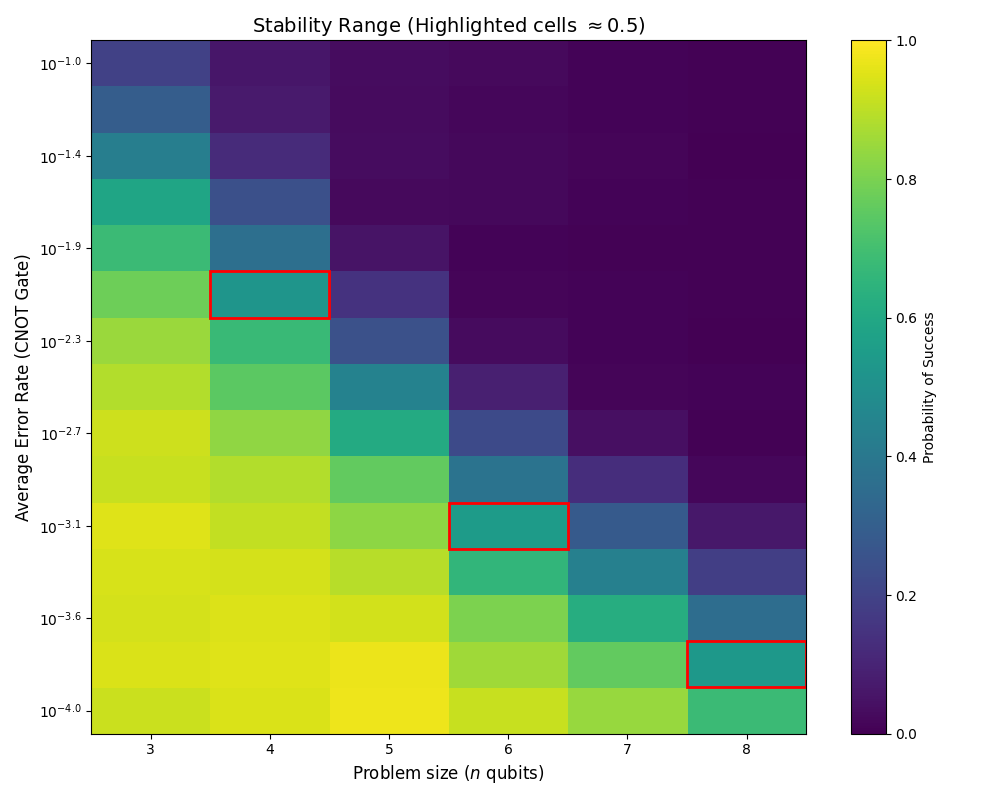
\includegraphics[width=\textwidth]{../asset/grover_heatmap_stability_range.png}
        \end{center}
    \end{columns}
\end{frame}

% ---------------------------------------------------------
% CONCLUSION
% ---------------------------------------------------------
\begin{frame}{Conclusion}
    \begin{itemize}
        \setlength\itemsep{1em}
        \item \textbf{Verification:} We successfully verified Grover's quadratic speedup and the ability to estimate $m$ via Quantum Counting.
        \item \textbf{Implementation Trade-offs:} Using Ancilla qubits is crucial on real hardware to keep circuit depth manageable.
        \item \textbf{Hardware Limits:} Noise analysis shows that Grover's algorithm requires deep circuits, making it challenging for current NISQ devices beyond small $n$.
    \end{itemize}
    
    \vspace{1cm}
    \centering \Large \textbf{Thank you for your attention.}
\end{frame}

\end{document}